\section{Introduction}
\label{sec:introduction}


% 1.videoQA overview-----------------------------------------
In name of the interactive AI, Video Question Answering (VideoQA) \cite{fan2019heterogeneous} has relished a overwhelming expansion in various domains, such as vision-language navigation and communication systems. 
%
To answer the natural language question based on the video content, the task \textit{per se} has bred multi-modal nature in its process of reasoning, which demands thorough comprehension across visual content and linguistic semantics.

% %
% Aiming to answer the natural language question based on the video content, Video Question Answering (VideoQA) \cite{fan2019heterogeneous} 
% has witnessed aggressive expansion in various domains, such as vision-language navigation and communication systems.
% To make the task intriguing, the multi-modal nature of VideoQA has bred interactive AI in its reasoning, which demands thorough comprehension across visual scenes and linguistic semantics.
%
% In this regard, various VidoeQA model realizes their excellence via a common paradigm of two modules:
% (1) \textit{video-question encoder} encapsulates the video content and the question semantics to representations;
% and (2) \textit{answer decoder} exploits the multi-modal representations to model the vision-language interaction and generate an answer. 

\begin{figure}[t]
\centering
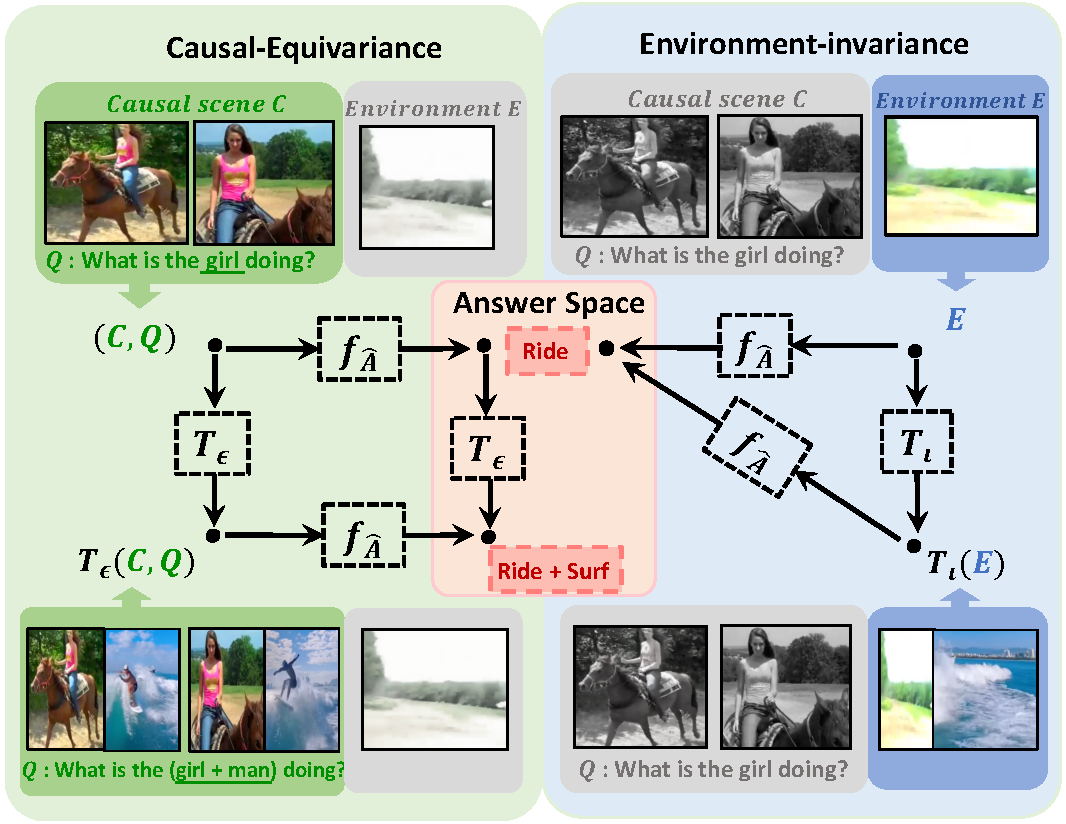
\includegraphics[scale=0.53]{fig/f1.pdf}
\caption{Illustration of causal-equivariant and environment-invariant principle, where $x$ is the model input, $f$ is a map from input space to answer space, $T$ is a transformation operator that applies to both input and answer space}.
% (\textcolor[rgb]{0,0.5,0}{Green}: causal-equivarince; \textcolor[rgb]{0.03,0.27,0.49}{Navy}: complement-invariance)}
\vspace{-5pt}
\label{fig:overview}
\end{figure}

% 2.problem of interpretable-------------------------------
Albeit the sterling performance, existing efforts usually express their reasoning mechanisms as black boxes. Unfortunately, peeping through their output does not reveal how machine leverage the multi-modal information, which refrains human intuition from machine intelligence and repels the nature of interactive AI. 
%the explanation of black-box models can provide insights into the relationship between input and output, thereby improving model design.
%shed light on model design
Worse still, overwhelming computational power has provoked the model complexity with billions of parameters, which, as a seed of distrust, shadowed the model's transparency along with our faith. 
%
Despite the necessity, the explainability of the current design still dwells on post-hoc visualization \cite{gao2018motionappearance,DBLP:conf/iccv/Liu0WL21,10.1145/3474085.3475620}, which is fragile against input perturbations, and less instructive to the predictive mechanism. 
%
% Clearly, inferring a reliable answer requires grounding rationale of the prediction, \ieto answer the million dollar question "which part of the video scene should be look at to answer the question". 
%
To the best of our knowledge, a self-interpretable VideoQA explainer that reveals the intrinsic prediction mechanism is critical to trustworthy videoQA but until-now lacking. 

% 3.partition the video to get interpretation ------------
Clearly, inferring a reliable answer requires a grounding rationale of the prediction, \ie to answer the million-dollar question "which part of the video scene should  be looking at?". 
%
Inspired by the information bottleneck, which tends to reduce the overload of information processing \cite{DBLP:conf/iclr/SaxeBDAKTC18}, we aim to find a shortcode for input video that preserves the maximum visual information toward the question, whose discovery will justify the prediction and increase the generalization. 
%
% Intuitively, filtering out task-irrelevant information reduces the overload of information processing, which naturally makes the representation more controllable.
%
Following this essence, one straightforward solution is to empower the model with discernment that splits the visual scene into two segments: 
(1) \textbf{causal scene} that retains the question-critical video content and preserving all the relevant information about the target answer, which naturally serves as interpretation for the prediction; (2) \textbf{environment scene} that holds answer-irrelevant environmental information of input video. 

% 4.euiqvariant and invariant for robust interpretation ---------------------------
% Modifying model's sensitivity to a certain transformation can have a substantial effect on the robustness of representation \cite{DBLP:journals/corr/abs-2111-00899}.
% %
% On top of the partition, one natural notion to acquire robust interpretation is making model sensitive to transformation of casual sense, while insensitive to transformation of complement sense.
% %
% Such philosophy of sensitivity is captured by the mathematical concept of equivariance and invariance: for a input$x$ and non-parametric transformation $T$, a encoder $f(.)$ is equivariant to $T$, if $∀x : f(T(x)) = T(f(x))$ ; Likewise, invariance is defined as $∀x : f(T(x)) = f(x)$.
% Specifically, the discovery of stable rationale implies two requirements on the partition:

%%%%%%
% Discovering  causal scene and answer is a luxury for videoQA without fine-grained supervision. 
Discovering causal scene without fine-grained supervision is a luxury for videoQA. Gazed upon the reasoning process, we argue crux of this problem is to amplify the connection between the causal scene and answer, while blocking the effect of environment. Following this line, we put forward \textit{Equivariance} and \textit{Invariance} principles to guide the partition learning.
% we borrow the mathematical concept of equivariance and invariance.
As shown in Figure \ref{fig:overview}, equivariance extends the model's sensitivity towards the a transformation $T$ on input $x$. Invariance, quite the contrary, inhibits the sensitivity and block model from input transformation. In light of this, the discovery of a stable rationale implies two requirements on the partition:
%
\begin{itemize}[leftmargin=*]
    \item \textbf{Causal-euqivariance.} In essence, transformation on the causal scene should cause the parallel change on the representation manifold. By introspecting ``How would the predictive answer vary if the causal scenes change?'', the grounding mechanism is aware of the transformations and thus maintains the predictive interpretation.
    In Figure \ref{fig:overview}, the euqivariance is exemplified in way that applying transformation $T$ to answer-critic information (\ie causal scene and question) should set off equivariant semantic change in answer space.
    In turn, a cautious formulation of such co-variation should helps the model to pinpoint the 'girl-on-horse' scene as grounding rationale for ``ride''.
    
    \item \textbf{Environmental-invariance.} On ground of the prophet, the answer prediction is invariant against permutation on environment scene, as it does not contribute to the reasoning mechanism or interpretation. 
    Consider the example in Figure \ref{fig:overview} again, since complement as ``landscape'' provide no evidence toward answer ``ride'', its corresponding transformation should reflect a homogeneity in the answer space. The invariance principle epitomizes such assumption by ruling a transformation that is in-vary to answer permutation.
\end{itemize}


%5.overall idea ------------------------------------------------------------------
Aspiring to capture grounding rationale, we formalize a model-agnostic learning framework, Equivariant and Invariant Grounding for Interpretable VideoQA (EGV), 
%
by asking the question ``what and how transformation should the model be equivariant or invariant to?'' 
%
Different from the previous effort that design supervised proxy task for geometric transformation \cite{DBLP:conf/iccv/ChengSM21}, 
% we adopted philosophy of causal intervention and design a saliency-aware temporal mix method for the video input, and impose 
we answer the ``what'' question by adopting the philosophy of causality \cite{pearl2009causal} and configure transformation as causal intervention operation that imposes scene-aware mixup \cite{DBLP:conf/iclr/ZhangCDL18} on the multi-modal input.
%
As for the question of how, we present a unified view of equivariant and invariant principles via the lens of temporal self-supervised learning, where the contrastive counterparts are bred through a disruption on the causal scene, environmental scene as well as vision-language alignment.

% where the contrastive counterparts are bred through a disruption on the causal and environmental scene, respectively.

% implemetation -----------------------------------------------------
In light of this idea, EGV absorbs three modules in addition to the backbone VideoQA model: a grounding indicator, an intervener, and a disruptor. 
%
In particular, the grounding indicator learns to separate the causal scenes as the interpretation and leave the rest as complement. Then the intervener performs a convex combination of two data points with different ratios on their causal and environmental parts. 
%
Noticeably, since mixing environment does not affect the reasoning dynamics, the answer is modified with the same ratio as the causal scene but independent to environmental one. 
%
By capturing the equivariance from the answer to the causal scene and the invariance to environment, the model perceives a faithful interpretation that preserves the predictive mechanism.
%
On top of the intervened video, the disruptor substitutes the complement scene with the stratification sampled from a memory bank (a collection of other training videos) and constitutes the “counterfactual video” as the positive sample.
Likewise, the negative sample is constructed via replacement on the causal scene. 
%
In addition to the visual negatives that ``disrupt'' the causal scene, the disruptor also develops alternatives by disrupting the visual-question coupling, to fortify their pair-wise cohesiveness.
% 
After acquiring anchor representation alongside its contrastive twins, the auxiliary contrastive objective reveals the discriminative representation purely from the scene of interest, thus fostering the robustness of interpretation.

Briefly put, our contributions are: 
\begin{itemize}[leftmargin=*]
    \item We proposed EGV, a model-agnostic VideoQA explainer that captures the intrinsic causal pattern in a self-interpretable manner.
    
    \item We investigate the soundness of grounding rationale by posing the equivariant-invariant principle on visual grounding and realize it via the causal instrument.
    
    \item We justify the superiority of EGV on three popular benchmark datasets (\ie MSVD-QA \cite{DBLP:conf/mm/XuZX0Z0Z17}, MSRVTT-QA \cite{DBLP:conf/mm/XuZX0Z0Z17},  NExT-QA \cite{DBLP:conf/cvpr/XiaoSYC21}) with extensive experiments, where our design outmatches all the state-of-the-art models.
\end{itemize}













